\section{Introduction}
\label{sec:Event}

Neuromorphic vision sensors, also known as \ac{DVS} \cite{lichtsteiner2008128x128} has been proposed as an effective alternative of vision sensor from its several advantages over regular cameras. Frame-based imaging sensors produce an image, which is time-synchronized scene data during exposure time. The sequential output known as image data is intuitive and effective for \ac{VO} \cite{forster2014svo} and \ac{SLAM} \cite{mur2017orb} even with a single camera. And the sensor measurement is produced by integrating a number of photons arrived during the exposure time, requiring specific duration for every measurement. Therefore, image data has limits of the trade-off between frame-rate and dynamic range and is not able to sense changes occurred in exposure time. However, event cameras are free from the problems of classic ones. Neuromorphic vision is not based on the number of photons integrated for a duration but measures the rate of a photon entering each pixel. Therefore, event cameras avoid temporal integration and retain asynchronicity with high dynamic range (up to $130dB$, which is significantly higher than the $60dB$ of conventional cameras).

Since the event camera possesses an asynchronous \ac{AER} representation of illumination change, data acquired from event cameras are not demonstrated with discrete timings. To fully utilize the unique \ac{AER} of event camera, any information obtained from the event camera should be dealt with as a continuous-time problem. However the number of events may sum up to millions per second, raising temporal sampling resolution does not solve the problem, yielding heavy computation load. Therefore event requires a total new way of data processing.

\begin{figure}%
	\centering%
	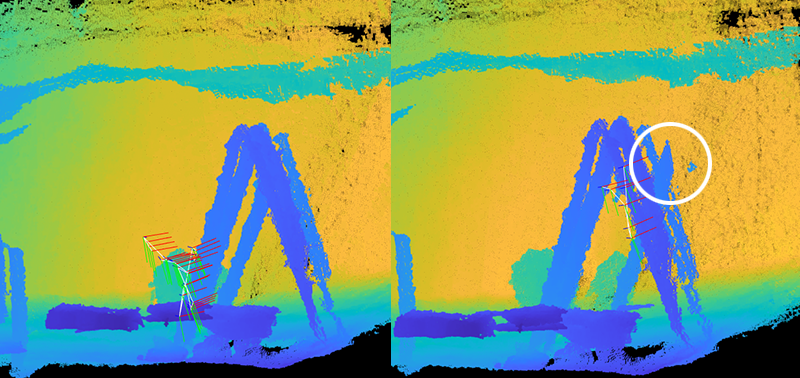
\includegraphics[width = \columnwidth]{figures/figure1small}%
	\captionsetup{justification=centering}
	\caption{Estimated trajectory and reconstruction from events \protect\linebreak with depth (left), Iterative
		Closest Points (ICP) on depth pointclouds (right). Trajectory estimation using only depth fails on extreme motion, as demonstrated in white circle.}%
	\label{F:main}%
	\vspace{-5mm}
\end{figure}

Thus event cameras related researches have focused on finding a way on processing temporal information while less degenerating data. Since pose representation enables global optimization techniques like bundle adjustment or pose-graph, majority of research in event-based \ac{VO} has been examined on transforming continuous signal into subsequent pose form \cite{lagorce2015asynchronous}, \cite{clady2015asynchronous}, \cite{weikersdorfer2012event}, \cite{kim2016real}. However, sequential procedures of classical image processing such as feature extraction, descriptor matching with calculating re-projection error were not necessary for event-based algorithms if the pose is not in a discrete representation \cite{rebecq2017evo} \cite{vidal2018ultimate}. Despite the idea of directly fitting motion from event measurements were in a proper way of utilizing the benefits of event cameras, its relatively lower spatial resolution and noise made it difficult to use events as a single origin pose estimator. To deal with this problem, we suggest combining sparse sensor measurements with events, while maintaining continuous pose representation as a trajectory.

In this paper, we aim to solve the motion estimation problem with the benefits of event sensors by:
%

\begin{itemize}
	\item Solving motion estimation problem by estimating polynomial spline trajectory from finding correspondence of continuous events between depth measurements

	\item Defining correspondence between events and disjointly updated depth, by associating depth discontinuity into event generating edges in the image domain.
	
	\item Releasing a first public dataset to cover illumination and motion variances by multi-modal sensor
	measurements consisted with event, depth, and thermal camera.

\end{itemize}

%---------------------------------------------------------------------------%
\section{Related Works}
\label{sec:related}

\subsection{Event-based Visual Odometry}

The unique advantages of \ac{AER} and event cameras have encouraged researchers to solve motion estimation aided by event measurements. Since event cameras have both advantages and challenges as described in the previous section, researchers have developed several ways of defining relationship between events, that are continuously measured but asynchronous to typical discrete pose representations.

In the early stages, researchers established probabilistic approaches on event-based \ac{VO}. A method that first succeeded involves calculating posterior probability with a temporal threshold. \citeauthor{kim2008simultaneous}~\cite{kim2008simultaneous} has introduced to use \ac{EM} schema on fitting events for upon rotational motion. This study was expanded to the optimization of 6-\ac{DOF} trajectory with 3D reconstruction \cite{kim2016real}. Their approach has revealed the way of directly optimizing the trajectory from events, yet was filter-based and had less robust due to numbers of assumptions. In \cite{weikersdorfer2012event}, authors implemented a particle filter to minimize ray distance through all features in 2D. This study was broadened to include 3D \ac{SLAM} in \cite{weikersdorfer2013simultaneous}, but was only effective in planar scenes.

On the other hand, there was another approach reminding of \ac{SAE} introduced in \cite{adelson1985spatiotemporal}. \cite{mueggler2015lifetime} fitted a surface in an $\mathcal{XYT}$ space with \ac{SAE} to estimate the effective temporal length for each event. These studies suggested finding the effective size of the temporal window and to only filter relevant events with adaptive temporal window size. The proposed algorithm provides a hint for utilizing the high temporal resolution characteristics of events by processing with individual timings.

In \cite{ieng2018neuromorphic}, a modified version of \ac{SAE} with exponentially decaying kernels was introduced for \ac{VO}. In this study, events are accumulated in exponential time-surface and calculated for an optimal camera pose by optimizing re-projection error with other measurement models in stereo-vision. The study focused on directly estimating the camera pose with exponentially decaying kernels, which provided a smoothed representation of \ac{SAE}. The authors introduced a robust descriptor of \ac{SAE} in addition to filtering with tree assignment. As a result, the author was able to enhance the mean tracking frequency on the scale. Although their work is based on the complex model and the user-defined descriptor, it has shown that calculating from each event's timestamp could arrange to a convergence.

The next was generating motion-related frame images by temporal thresholding. Numbers of researches had set effective events within a fixed time interval and tried to build event images for discrete trajectory estimation. However, this procedure integrates the asynchronous event signals into synchronous sequences with a fixed temporal window, resulting in the loss of piecewise timing information on each event. Therefore in order to achieve higher levels of accuracy and fully utilize the temporal resolution of event cameras, another solution were required than simple thresholding.

Several studies attempted to utilize the high temporal resolution of event cameras by assigning proper weights to each event. \citeauthor{gallego2017accurate}~\cite{gallego2017accurate} introduced a direct method of accurately estimating angular velocity by compensating events for rotational motion. This approach was the first attempt to build a motion-compensated event frame, that could both conserve asynchronicity and frame-based odometry estimation. In combination with nonlinear optimization, \cite{rebecq2017real} succeeded in integrating \ac{IMU} for 6 \ac{DOF} event \ac{VO}. This study demonstrated a standard pipeline for event-based \ac{VINS}. Although this approach became robust and effective by enabling classical feature-based methods on an event stream, the requirement of generation procedure on the motion-compensated event image for every pose and extracting features demands proper initialization.

\citeauthor{mueggler2018continuous}~\cite{mueggler2018continuous} proposed a method of optimizing the trajectory with events and \ac{IMU} by introducing cubic spline interpolation into \cite{rebecq2017evo}. Ultimate SLAM \cite{vidal2018ultimate} was nonetheless the state-of-the-art method for integrating sensor measurements with motion-compensated event frames. However, the proposed algorithm required updating the spline parameter upon receiving each event, which was quite heavy in computation.

In this research, we introduce a method to estimate polynomial continuous trajectory in 3D,
by directly optimizing spline parameters efficiently with continuous event measurements and
sparsely obtained depth measurements.

\subsection{Datasets for Environmental Variance}

Numbers of datasets for benchmarking \ac{SLAM} has been introduced
\cite{Cordts2016Cityscapes}, \cite{jjeong-2019-ijrr} with
clear sight and high visibility. Meanwhile, in the real world, lighting
conditions are often uncooperative, making computer vision algorithms fail.
Moreover, there are few of datasets made to test experimental
environments with environmental variations.

NCLT \cite{ncarlevaris-2015a} and TUM MonoVO \cite{engel2016photometrically}
introduced large scale data with huge variance in environments for long-term visual
\ac{SLAM}. These datasets cover challenging indoor and outdoor sequences including
natural light and weather changes. However, obtaining the limited information from the
classical camera restricts the bandwidth of data from the environment, skipping
potentially important information.

By using other types of visual sensors, Choi et al. \cite{8293689} presented
a multi-spectral day/night dataset with the sensor set of stereo RGB, LiDAR and
a thermal camera. Their data contains variance along the whole day. Furthermore,
numbers of labeled data are provided for autonomous navigation.
However, camera movements in the dataset are limited to planar motion because the
system is mounted on a car.

In \cite{zhu2018multivehicle}, the authors have presented a dataset measuring
various lighting and motion sequences with two event cameras aligned with
inertial sensors and an \ac{IMU}. The dataset contains a large variety of
condition changes, suggesting utilizing the event camera for low latency and high
dynamic range characteristics.

Although several datasets have contained environmental variations
including movement or lighting variances, unspecified natural environment often
possess both of them. In this paper, we release a dataset to record both thermal
and events with depth in order to deal with two significant disturbances:
luminance conditions and motion. Along the dataset, we also suggest the method to
estimate polynomial continuous trajectory in 3D, thereby directly optimizing spline\
parameters efficiently with given depth measurements.
